\documentclass{article}
\def\xcolorversion{2.00}
\def\xkeyvalversion{1.8}

\usepackage[version=0.96]{pgf}
\usepackage{tikz}
\usetikzlibrary{arrows,shapes,snakes,automata,backgrounds,petri,calc}
\usepackage[latin1]{inputenc}
\usepackage{verbatim}
\usepackage{color}
\usepackage{graphicx}

\definecolor{jlabRed}{HTML}{C0272D}
\definecolor{jlabOrange}{HTML}{F96600}
\definecolor{jlabBlue}{HTML}{2F7A79}
\definecolor{jlabGreen}{HTML}{417D0A}
\definecolor{jlabLightGray}{HTML}{E5E5E5}
\definecolor{betterLightGray}{HTML}{A7A7A7}
\definecolor{jlabPurple}{HTML}{800080}
\definecolor{jlabDarkGray}{HTML}{7D8288} 


\begin{document}
\pagestyle{empty}

\hspace*{-4.5cm}{
  \begin{tikzpicture}[>=stealth']

    \node[anchor=south west] (Plot) at (1,7) 
      {
        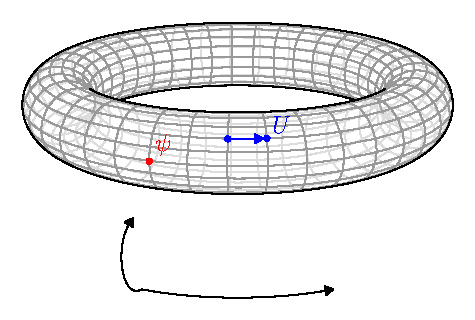
\includegraphics[scale=1,trim=0cm 0cm 0cm 0cm,clip]{lattice.pdf}
      };

    %% markups 

	\node (l1) at (5,7.2) { \small $t$}; 
	\node (l1) at (3,8.1) { \small $x$}; 


    % \draw[help lines, xstep = 1, ystep = 1] (0,0) grid (15,17);

  \end{tikzpicture}
} % fbox









\end{document}
